\documentclass[aspectratio=169,9pt]{beamer}

\usepackage{graphicx,caption,subcaption,hyperref,amsmath,tikz}
\graphicspath{ {./figures/} }
\captionsetup{font=scriptsize,labelfont=scriptsize}
\setbeamerfont{footnote}{size=\scriptsize}
\usepackage[strict]{changepage}
\usetikzlibrary{arrows,automata,positioning}
\usetheme[titleformat=smallcaps,
            sectionpage=progressbar,
			subsectionpage=progressbar,
			progressbar=frametitle,
			numbering=fraction]{metropolis}
% \usecolortheme{owl}
\usepackage[style=apa,
			sorting=nyt,
			date=year,
			bibencoding=utf8,
			isbn=false,
			eprint=false,
			dashed=false,
			uniquelist=false,
			maxbibnames=10,
			minbibnames=1,
			maxcitenames=2,
			uniquename=init,
			giveninits=true,
			useprefix=false,
			minsortnames=1,
			maxsortnames=2]{biblatex}
\bibliography{References}

% Information to be included in the title page:
\title{Deciphering the landscape of cell states in Glioblastoma}
\author{Harshavardhan BV}
\date{\today}
\institute{IISc Bangalore}

\begin{document}
    \frame{\titlepage}
    \section{Introduction}

    \begin{frame}{Molecular subtypes of GBM}
        \begin{adjustwidth}{-5cm}{-5cm}
            \centering
            \begin{figure}
                \centering
                \begin{subfigure}{0.4\textwidth}
                    \centering
                    \includegraphics[width=\textwidth]{neftel_ninja_star}
                    \caption{Cell states by \cite{Neftel}}
                \end{subfigure}
                \pause
                \begin{subfigure}{0.6\textwidth}
                    \centering
                    \includegraphics[width=\textwidth]{verhaak_clusters}
                    \caption{Cell states by \cite{Verhaak}}
                \end{subfigure}
                \pause[1]\caption{Cellular states defined for Glioblastoma}
            \end{figure}
        \end{adjustwidth}
    \end{frame}

    \begin{frame}[standout]
        Are these cell states distinct?
        
        \pause How does this heterogeneity and plasticity affect therapy?
    \end{frame}

    \begin{frame}{Datasets}
    \begin{table}[]
        \centering
        \begin{tabular}{|l|l|l|l|}
            \hline
            \textbf{Dataset} & \textbf{CellLine/Tumour} & \textbf{Bulk/SingleCell} & \textbf{Source}\\ \hline
            CCLE             & CellLine                 & Bulk                     & \cite{CCLE}\\ \hline
            TCGA             & Tumour                   & Bulk                     & \cite{TCGA-GBM}\\ \hline
            GSE131928        & Tumour                   & SingleCell               & \cite{Neftel}  \\ \hline
            GSE168004        & CellLine                 & SingleCell               & \cite{scCL_GBM}\\ \hline
%             GSE182109        & Tumour                   & SingleCell               \\ \hline
            \end{tabular}
    \end{table}
    \end{frame}

    \section{Preliminary results}
    \begin{frame}{Gene-set enrichment - Neftel et al}
        \begin{adjustwidth}{-5cm}{-5cm}
            \centering
            \begin{figure}
                \centering
                \begin{subfigure}[c]{0.48\textwidth}
                    \centering
                    \includegraphics[width=\textwidth]{ssGSEA_CCLE_corrplot_Nef}
                    \caption{CCLE (Bulk-CellLine)}
                \end{subfigure}
                \begin{subfigure}[c]{0.48\textwidth}
                    \centering
                    \includegraphics[width=\textwidth]{ssGSEA_TCGA_corrplot_Nef}
                    \caption{TCGA (Bulk-Tumour)}
                \end{subfigure}
                \caption{Correlation of ssGSEA scores - Neftel}
            \end{figure}
        \end{adjustwidth}
    \end{frame}

    \begin{frame}{Gene-set enrichment - Neftel et al}
        \begin{adjustwidth}{-5cm}{-5cm}
            \centering
            \begin{figure}\ContinuedFloat
                \centering
                \begin{subfigure}[c]{0.48\textwidth}
                    \centering
                    \includegraphics[width=\textwidth]{AUCell_GSM3828672_corrplot_Nef}
                    \caption{GSE131928 (SingleCell-Tumour)}
                \end{subfigure}
                \begin{subfigure}[c]{0.48\textwidth}
                    \centering
                    \includegraphics[width=\textwidth]{AUCell_mgg23_corrplot_Nef}
                    \caption{GSE168004 (SingleCell-CellLine)}
                \end{subfigure}
                \caption{Correlation of AUCell scores - Neftel}
            \end{figure}
        \end{adjustwidth}
    \end{frame}

    \begin{frame}{Gene-set enrichment - Verhaak et al}
        \begin{adjustwidth}{-5cm}{-5cm}
            \centering
            \begin{figure}\ContinuedFloat
                \centering
                \begin{subfigure}[c]{0.48\textwidth}
                    \centering
                    \includegraphics[width=\textwidth]{ssGSEA_CCLE_corrplot_Ver}
                    \caption{CCLE (Bulk-CellLine)}
                \end{subfigure}
                \begin{subfigure}[c]{0.48\textwidth}
                    \centering
                    \includegraphics[width=\textwidth]{ssGSEA_TCGA_corrplot_Ver}
                    \caption{TCGA (Bulk-Tumour)}
                \end{subfigure}
                \caption{Correlation of ssGSEA scores - Verhaak}
            \end{figure}
        \end{adjustwidth}
    \end{frame}

    \begin{frame}{Gene-set enrichment - Verhaak et al}
        \begin{adjustwidth}{-5cm}{-5cm}
            \centering
            \begin{figure}\ContinuedFloat
                \centering
                \begin{subfigure}[c]{0.48\textwidth}
                    \centering
                    \includegraphics[width=\textwidth]{AUCell_GSM3828672_corrplot_Ver}
                    \caption{GSE131928 (SingleCell-Tumour)}
                \end{subfigure}
                \begin{subfigure}[c]{0.48\textwidth}
                    \centering
                    \includegraphics[width=\textwidth]{AUCell_mgg23_corrplot_Ver}
                    \caption{GSE168004 (SingleCell-CellLine)}
                \end{subfigure}
                \caption{Correlation of AUCell scores - Verhaak}
            \end{figure}
        \end{adjustwidth}
    \end{frame}

    \begin{frame}{Gene-set enrichment - Comparison}
        \begin{adjustwidth}{-5cm}{-5cm}
            \centering
            \begin{figure}\ContinuedFloat
                \centering
                \begin{subfigure}[c]{0.48\textwidth}
                    \centering
                    \includegraphics[width=\textwidth]{ssGSEA_CCLE_corrplot_2D}
                    \caption{CCLE (Bulk-CellLine)}
                \end{subfigure}
                \begin{subfigure}[c]{0.48\textwidth}
                    \centering
                    \includegraphics[width=\textwidth]{ssGSEA_TCGA_corrplot_2D}
                    \caption{TCGA (Bulk-Tumour)}
                \end{subfigure}
                \caption{Correlation of ssGSEA scores - Comparison}
            \end{figure}
        \end{adjustwidth}
    \end{frame}

    \begin{frame}{Gene-set enrichment - Comparison}
        \begin{adjustwidth}{-5cm}{-5cm}
            \centering
            \begin{figure}\ContinuedFloat
                \centering
                \begin{subfigure}[c]{0.48\textwidth}
                    \centering
                    \includegraphics[width=\textwidth]{AUCell_GSM3828672_corrplot_2D}
                    \caption{GSE131928 (SingleCell-Tumour)}
                \end{subfigure}
                \begin{subfigure}[c]{0.48\textwidth}
                    \centering
                    \includegraphics[width=\textwidth]{AUCell_mgg23_corrplot_2D}
                    \caption{GSE168004 (SingleCell-CellLine)}
                \end{subfigure}
                \caption{Correlation of AUCell scores- Comparison}
            \end{figure}
        \end{adjustwidth}
    \end{frame}
    
    \begin{frame}{Signatures}
        \begin{adjustwidth}{-5cm}{-5cm}
            \centering
            \begin{figure}
                \centering
                \begin{subfigure}[c]{0.38\textwidth}
                    \centering
                    \includegraphics[width=\textwidth]{signature_overlap_Nef}
                    \caption{Neftel et al signature}
                \end{subfigure}
                \pause
                \begin{subfigure}[c]{0.38\textwidth}
                    \centering
                    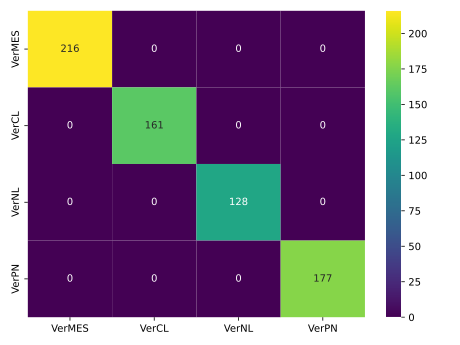
\includegraphics[width=\textwidth]{signature_overlap_Ver}
                    \caption{Verhaak et al signature}
                \end{subfigure}
                \pause
                \begin{subfigure}[c]{0.38\textwidth}
                    \centering
                    \includegraphics[width=\textwidth]{signature_overlap_All}
                    \caption{Signature of both}
                \end{subfigure}
                \pause[1]\caption{Overlap of genes in the signatures}
            \end{figure}
        \end{adjustwidth}
    \end{frame}

    \begin{frame}{Signatures}
        \begin{table}[]
            \centering
            \resizebox{\textwidth}{!}{%
                \begin{tabular}{|l|llllllll|}
                    \hline
                    \textbf{NefNPC-VerPN}  & ABAT  & AMOTL2 & ASCL1  & BCAN  & BEX1 & CHD7 & DBN1 & DCX \\
                    & DLL3 & FXYD6   & MAP2  & MARCKSL1 & MLLT11 & MYT1 & PAK3 & PFN2 \\
                    & SCG3 & SEZ6L & SOX11 & SOX4 & STMN1 & STMN4 & & \\ \hline
                    \textbf{NefMES-VerMES} & ANXA1 & ANXA2  & CHI3L1 & CLIC1 & CTSB & EMP3 & LGALS1 & LGALS3 \\
                    & NPC2 & S100A11 & SERPINE1 & TIMP1    & TNFRSF1A & WWTR1 & & \\ \hline
                \end{tabular}%
            }
            \caption{Genes common between signatures}
        \end{table}
    \end{frame}

    \begin{frame}{Signature Expression - Neftel et al}
        \begin{adjustwidth}{-5cm}{-5cm}
            \centering
            \begin{figure}
                \centering
                \begin{subfigure}[c]{0.48\textwidth}
                    \centering
                    \includegraphics[width=\textwidth]{CCLE_Corrplot_Nef}
                    \caption{CCLE (Bulk-CellLine)}
                \end{subfigure}
                \begin{subfigure}[c]{0.48\textwidth}
                    \centering
                    \includegraphics[width=\textwidth]{TCGA_Corrplot_Nef}
                    \caption{TCGA (Bulk-Tumour)}
                \end{subfigure}
                \caption{Correlation of signature expression - Neftel}
            \end{figure}
        \end{adjustwidth}
    \end{frame}

    \begin{frame}{Signature Expression - Neftel et al}
        \begin{adjustwidth}{-5cm}{-5cm}
            \centering
            \begin{figure}\ContinuedFloat
                \centering
                \begin{subfigure}[c]{0.48\textwidth}
                    \centering
                    \includegraphics[width=\textwidth]{GSM3828672_Corrplot_Nef}
                    \caption{GSE131928 (SingleCell-Tumour)}
                \end{subfigure}
                \begin{subfigure}[c]{0.48\textwidth}
                    \centering
                    \includegraphics[width=\textwidth]{mgg23_Corrplot_Nef}
                    \caption{GSE168004 (SingleCell-CellLine)}
                \end{subfigure}
                \caption{Correlation of signature expression - Neftel}
            \end{figure}
        \end{adjustwidth}
    \end{frame}


    \begin{frame}{Signature Expression - Verhaak et al}
        \begin{adjustwidth}{-5cm}{-5cm}
            \centering
            \begin{figure}\ContinuedFloat
                \centering
                \begin{subfigure}[c]{0.48\textwidth}
                    \centering
                    \includegraphics[width=\textwidth]{CCLE_Corrplot_Ver}
                    \caption{CCLE (Bulk-CellLine)}
                \end{subfigure}
                \begin{subfigure}[c]{0.48\textwidth}
                    \centering
                    \includegraphics[width=\textwidth]{TCGA_Corrplot_Ver}
                    \caption{TCGA (Bulk-Tumour)}
                \end{subfigure}
                \caption{Correlation of signature expression - Verhaak}
            \end{figure}
        \end{adjustwidth}
    \end{frame}

    \begin{frame}{Signature Expression - Verhaak et al}
        \begin{adjustwidth}{-5cm}{-5cm}
            \centering
            \begin{figure}\ContinuedFloat
                \centering
                \begin{subfigure}[c]{0.48\textwidth}
                    \centering
                    \includegraphics[width=\textwidth]{GSM3828672_Corrplot_Ver}
                    \caption{GSE131928 (SingleCell-Tumour)}
                \end{subfigure}
                \begin{subfigure}[c]{0.48\textwidth}
                    \centering
                    \includegraphics[width=\textwidth]{mgg23_Corrplot_Ver}
                    \caption{GSE168004 (SingleCell-CellLine)}
                \end{subfigure}
                \caption{Correlation of signature expression - Verhaak}
            \end{figure}
        \end{adjustwidth}
    \end{frame}

    \begin{frame}{Pairwise Signature Expression - Metric}
        $$Consistency = \frac{1}{2}(\frac{\sum_{x,y \in S_1, S_1} \rho_R(x,y)}{2 (N_1)^2} + \frac{\sum_{x,y \in S_2, S_2} \rho_R(x,y)}{2 (N_2)^2} - \frac{\sum_{x,y \in S_1, S_2} \rho_R(x,y)}{N_1 N_2})$$
        {\footnotesize Where,
        \begin{itemize}
            \item $\rho_R(x,y)$ = Spearman correlation between x and y
            \item $S_i$ = Signature i
            \item $N_i$ = No. of genes in Signature i
        \end{itemize}}
        \pause
        \begin{adjustwidth}{-5cm}{-5cm}
            \centering
            \begin{figure}
                \centering
                \begin{subfigure}[c]{0.5\textwidth}
                    \centering
                    \includegraphics[width=0.5\textwidth]{strong_teams}
                    \caption{Consistency = 1}
                \end{subfigure}
                \begin{subfigure}[c]{0.5\textwidth}
                    \centering
                    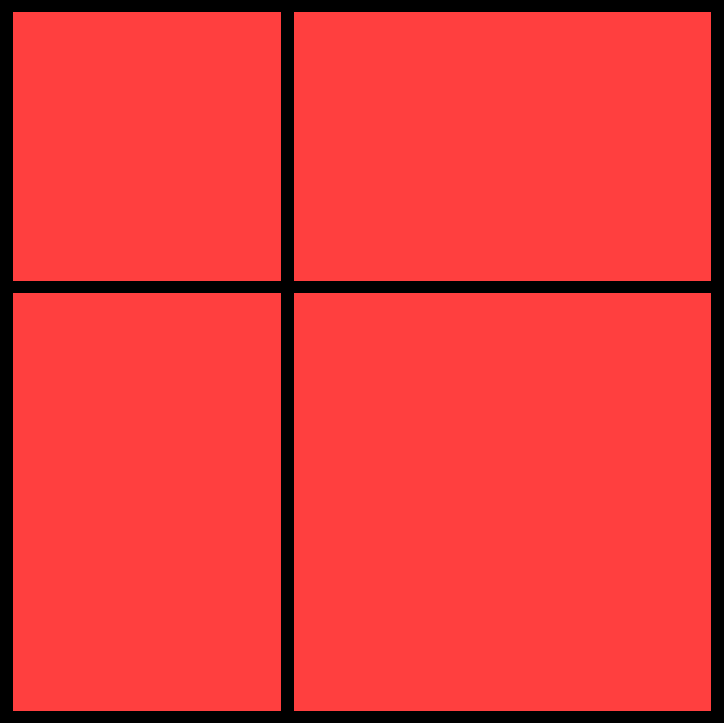
\includegraphics[width=0.5\textwidth]{no_teams}
                    \caption{Consistency = 0}
                \end{subfigure}
                \caption{Consistency on example cases}
            \end{figure}
        \end{adjustwidth}
    \end{frame}

    \begin{frame}{Pairwise Signature Expression - Neftel et al}
        \begin{adjustwidth}{-5cm}{-5cm}
            \centering
            \begin{figure}
                \centering
                \begin{subfigure}[c]{0.7\textwidth}
                    \centering
                    \includegraphics[width=\textwidth]{CCLE_Corrplot_pair-Nef}
                    \caption{Pairwise Signature Correlation}
                \end{subfigure}
                \begin{subfigure}[c]{0.4\textwidth}
                    \centering
                    \includegraphics[width=\textwidth]{CCLE_Consistency_Nef}
                    \caption{Consistency of Signature Correlation}
                \end{subfigure}
                \caption{Pairwise correlation of signature expression - CCLE (Bulk-CellLine) - Neftel}
            \end{figure}
        \end{adjustwidth}
    \end{frame}

    \begin{frame}{Pairwise Signature Expression - Verhaak et al}
        \begin{adjustwidth}{-5cm}{-5cm}
            \centering
            \begin{figure}\ContinuedFloat
                \centering
                \begin{subfigure}[c]{0.7\textwidth}
                    \centering
                    \includegraphics[width=\textwidth]{CCLE_Corrplot_pair-Ver}
                    \caption{Pairwise Signature Correlation}
                \end{subfigure}
                \begin{subfigure}[c]{0.4\textwidth}
                    \centering
                    \includegraphics[width=\textwidth]{CCLE_Consistency_Ver}
                    \caption{Consistency of Signature Correlation}
                \end{subfigure}
                \caption{Pairwise correlation of signature expression - CCLE (Bulk-CellLine) - Verhaak}
            \end{figure}
        \end{adjustwidth}
    \end{frame}

    \begin{frame}{Pairwise Signature Expression - Comparison}
        \begin{adjustwidth}{-5cm}{-5cm}
            \centering
            \begin{figure}\ContinuedFloat
                \centering
                \begin{subfigure}[c]{0.7\textwidth}
                    \centering
                    \includegraphics[width=\textwidth]{CCLE_Corrplot_pair-Mix}
                    \caption{Pairwise Signature Correlation}
                \end{subfigure}
                \begin{subfigure}[c]{0.4\textwidth}
                    \centering
                    \includegraphics[width=\textwidth]{CCLE_Consistency_Mix}
                    \caption{Consistency of Signature Correlation}
                \end{subfigure}
                \caption{Pairwise correlation of signature expression - CCLE (Bulk-CellLine) - Comparison}
            \end{figure}
        \end{adjustwidth}
    \end{frame}

    \begin{frame}{Pairwise Signature Expression - Neftel et al}
        \begin{adjustwidth}{-5cm}{-5cm}
            \centering
            \begin{figure}
                \centering
                \begin{subfigure}[c]{0.7\textwidth}
                    \centering
                    \includegraphics[width=\textwidth]{TCGA_Corrplot_pair-Nef}
                    \caption{Pairwise Signature Correlation}
                \end{subfigure}
                \begin{subfigure}[c]{0.4\textwidth}
                    \centering
                    \includegraphics[width=\textwidth]{TCGA_Consistency_Nef}
                    \caption{Consistency of Signature Correlation}
                \end{subfigure}
                \caption{Pairwise correlation of signature expression - TCGA (Bulk-Tumour) - Neftel}
            \end{figure}
        \end{adjustwidth}
    \end{frame}

    \begin{frame}{Pairwise Signature Expression - Verhaak et al}
        \begin{adjustwidth}{-5cm}{-5cm}
            \centering
            \begin{figure}\ContinuedFloat
                \centering
                \begin{subfigure}[c]{0.7\textwidth}
                    \centering
                    \includegraphics[width=\textwidth]{TCGA_Corrplot_pair-Ver}
                    \caption{Pairwise Signature Correlation}
                \end{subfigure}
                \begin{subfigure}[c]{0.4\textwidth}
                    \centering
                    \includegraphics[width=\textwidth]{TCGA_Consistency_Ver}
                    \caption{Consistency of Signature Correlation}
                \end{subfigure}
                \caption{Pairwise correlation of signature expression - TCGA (Bulk-Tumour) - Verhaak}
            \end{figure}
        \end{adjustwidth}
    \end{frame}

    \begin{frame}{Pairwise Signature Expression - Comparison}
        \begin{adjustwidth}{-5cm}{-5cm}
            \centering
            \begin{figure}\ContinuedFloat
                \centering
                \begin{subfigure}[c]{0.7\textwidth}
                    \centering
                    \includegraphics[width=\textwidth]{TCGA_Corrplot_pair-Mix}
                    \caption{Pairwise Signature Correlation}
                \end{subfigure}
                \begin{subfigure}[c]{0.4\textwidth}
                    \centering
                    \includegraphics[width=\textwidth]{TCGA_Consistency_Mix}
                    \caption{Consistency of Signature Correlation}
                \end{subfigure}
                \caption{Pairwise correlation of signature expression - TCGA (Bulk-Tumour) - Comparison}
            \end{figure}
        \end{adjustwidth}
    \end{frame}


    \begin{frame}{Pairwise Signature Expression - Neftel et al}
        \begin{adjustwidth}{-5cm}{-5cm}
            \centering
            \begin{figure}
                \centering
                \begin{subfigure}[c]{0.7\textwidth}
                    \centering
                    \includegraphics[width=\textwidth]{GSM3828672_Corrplot_pair-Nef}
                    \caption{Pairwise Signature Correlation}
                \end{subfigure}
                \begin{subfigure}[c]{0.4\textwidth}
                    \centering
                    \includegraphics[width=\textwidth]{GSM3828672_Consistency_Nef}
                    \caption{Consistency of Signature Correlation}
                \end{subfigure}
                \caption{Pairwise correlation of signature expression - GSE131928 (SingleCell-Tumour) - Neftel}
            \end{figure}
        \end{adjustwidth}
    \end{frame}

    \begin{frame}{Pairwise Signature Expression - Verhaak et al}
        \begin{adjustwidth}{-5cm}{-5cm}
            \centering
            \begin{figure}\ContinuedFloat
                \centering
                \begin{subfigure}[c]{0.7\textwidth}
                    \centering
                    \includegraphics[width=\textwidth]{GSM3828672_Corrplot_pair-Ver}
                    \caption{Pairwise Signature Correlation}
                \end{subfigure}
                \begin{subfigure}[c]{0.4\textwidth}
                    \centering
                    \includegraphics[width=\textwidth]{GSM3828672_Consistency_Ver}
                    \caption{Consistency of Signature Correlation}
                \end{subfigure}
                \caption{Pairwise correlation of signature expression - GSE131928 (SingleCell-Tumour) - Verhaak}
            \end{figure}
        \end{adjustwidth}
    \end{frame}

    \begin{frame}{Pairwise Signature Expression - Comparison}
        \begin{adjustwidth}{-5cm}{-5cm}
            \centering
            \begin{figure}\ContinuedFloat
                \centering
                \begin{subfigure}[c]{0.7\textwidth}
                    \centering
                    \includegraphics[width=\textwidth]{GSM3828672_Corrplot_pair-Mix}
                    \caption{Pairwise Signature Correlation}
                \end{subfigure}
                \begin{subfigure}[c]{0.4\textwidth}
                    \centering
                    \includegraphics[width=\textwidth]{GSM3828672_Consistency_Mix}
                    \caption{Consistency of Signature Correlation}
                \end{subfigure}
                \caption{Pairwise correlation of signature expression - GSE131928 (SingleCell-Tumour) - Comparison}
            \end{figure}
        \end{adjustwidth}
    \end{frame}

    \begin{frame}{Pairwise Signature Expression - Neftel et al}
        \begin{adjustwidth}{-5cm}{-5cm}
            \centering
            \begin{figure}
                \centering
                \begin{subfigure}[c]{0.7\textwidth}
                    \centering
                    \includegraphics[width=\textwidth]{mgg23_Corrplot_pair-Nef}
                    \caption{Pairwise Signature Correlation}
                \end{subfigure}
                \begin{subfigure}[c]{0.4\textwidth}
                    \centering
                    \includegraphics[width=\textwidth]{mgg23_Consistency_Nef}
                    \caption{Consistency of Signature Correlation}
                \end{subfigure}
                \caption{Pairwise correlation of signature expression - GSE168004 (SingleCell-CellLine) - Neftel}
            \end{figure}
        \end{adjustwidth}
    \end{frame}

    \begin{frame}{Pairwise Signature Expression - Verhaak et al}
        \begin{adjustwidth}{-5cm}{-5cm}
            \centering
            \begin{figure}\ContinuedFloat
                \centering
                \begin{subfigure}[c]{0.7\textwidth}
                    \centering
                    \includegraphics[width=\textwidth]{mgg23_Corrplot_pair-Ver}
                    \caption{Pairwise Signature Correlation}
                \end{subfigure}
                \begin{subfigure}[c]{0.4\textwidth}
                    \centering
                    \includegraphics[width=\textwidth]{mgg23_Consistency_Ver}
                    \caption{Consistency of Signature Correlation}
                \end{subfigure}
                \caption{Pairwise correlation of signature expression - GSE168004 (SingleCell-CellLine) - Verhaak}
            \end{figure}
        \end{adjustwidth}
    \end{frame}

    \begin{frame}{Pairwise Signature Expression - Comparison}
        \begin{adjustwidth}{-5cm}{-5cm}
            \centering
            \begin{figure}\ContinuedFloat
                \centering
                \begin{subfigure}[c]{0.7\textwidth}
                    \centering
                    \includegraphics[width=\textwidth]{mgg23_Corrplot_pair-Mix}
                    \caption{Pairwise Signature Correlation}
                \end{subfigure}
                \begin{subfigure}[c]{0.4\textwidth}
                    \centering
                    \includegraphics[width=\textwidth]{mgg23_Consistency_Mix}
                    \caption{Consistency of Signature Correlation}
                \end{subfigure}
                \caption{Pairwise correlation of signature expression - GSE168004 (SingleCell-CellLine) - Comparison}
            \end{figure}
        \end{adjustwidth}
    \end{frame}

    \begin{frame}{PCA of Signature - Neftel et al}
        \begin{adjustwidth}{-5cm}{-5cm}
            \centering
            \begin{figure}
                \centering
                \begin{subfigure}[c]{0.48\textwidth}
                    \centering
                    \includegraphics[width=\textwidth]{CCLE_loadings_barplot_Nef}
                    \caption{CCLE (Bulk-CellLine)}
                \end{subfigure}
                \begin{subfigure}[c]{0.48\textwidth}
                    \centering
                    \includegraphics[width=\textwidth]{TCGA_loadings_barplot_Nef}
                    \caption{TCGA (Bulk-Tumour)}
                \end{subfigure}
                \caption{Loadings of PC1 - PCA on signature expression - Neftel}
            \end{figure}
        \end{adjustwidth}
    \end{frame}

    \begin{frame}{PCA of Signature - Neftel et al}
        \begin{adjustwidth}{-5cm}{-5cm}
            \centering
            \begin{figure}\ContinuedFloat
                \centering
                \begin{subfigure}[c]{0.48\textwidth}
                    \centering
                    \includegraphics[width=\textwidth]{GSM3828672_loadings_barplot_Nef}
                    \caption{GSE131928 (SingleCell-Tumour)}
                \end{subfigure}
                \begin{subfigure}[c]{0.48\textwidth}
                    \centering
                    \includegraphics[width=\textwidth]{mgg23_loadings_barplot_Nef}
                    \caption{GSE168004 (SingleCell-CellLine)}
                \end{subfigure}
                \caption{Loadings of PC1 - PCA on signature expression - Neftel}
            \end{figure}
        \end{adjustwidth}
    \end{frame}

    \begin{frame}{PCA of Signature - Verhaak et al}
        \begin{adjustwidth}{-5cm}{-5cm}
            \centering
            \begin{figure}\ContinuedFloat
                \centering
                \begin{subfigure}[c]{0.48\textwidth}
                    \centering
                    \includegraphics[width=\textwidth]{CCLE_loadings_barplot_Ver}
                    \caption{CCLE (Bulk-CellLine)}
                \end{subfigure}
                \begin{subfigure}[c]{0.48\textwidth}
                    \centering
                    \includegraphics[width=\textwidth]{TCGA_loadings_barplot_Ver}
                    \caption{TCGA (Bulk-Tumour)}
                \end{subfigure}
                \caption{Loadings of PC1 - PCA on signature expression - Verhaak}
            \end{figure}
        \end{adjustwidth}
    \end{frame}

    \begin{frame}{PCA of Signature - Verhaak et al}
        \begin{adjustwidth}{-5cm}{-5cm}
            \centering
            \begin{figure}\ContinuedFloat
                \centering
                \begin{subfigure}[c]{0.48\textwidth}
                    \centering
                    \includegraphics[width=\textwidth]{GSM3828672_loadings_barplot_Ver}
                    \caption{GSE131928 (SingleCell-Tumour)}
                \end{subfigure}
                \begin{subfigure}[c]{0.48\textwidth}
                    \centering
                    \includegraphics[width=\textwidth]{mgg23_loadings_barplot_Ver}
                    \caption{GSE168004 (SingleCell-CellLine)}
                \end{subfigure}
                \caption{Loadings of PCA on signature expression - Verhaak}
            \end{figure}
        \end{adjustwidth}
    \end{frame}

    \begin{frame}{PCA vs Gene-sets - Neftel et al}
        \begin{adjustwidth}{-5cm}{-5cm}
            \centering
            \begin{figure}
                \centering
                \begin{subfigure}[c]{0.48\textwidth}
                    \centering
                    \includegraphics[width=\textwidth]{CCLE_load-corr_Nef}
                    \caption{CCLE (Bulk-CellLine)}
                \end{subfigure}
                \begin{subfigure}[c]{0.48\textwidth}
                    \centering
                    \includegraphics[width=\textwidth]{TCGA_load-corr_Nef}
                    \caption{TCGA (Bulk-Tumour)}
                \end{subfigure}
                \caption{Correlation of top loadings of PCA with ssGSEA scores - Neftel}
            \end{figure}
        \end{adjustwidth}
    \end{frame}

    \begin{frame}{PCA vs Gene-sets - Neftel et al}
        \begin{adjustwidth}{-5cm}{-5cm}
            \centering
            \begin{figure}\ContinuedFloat
                \centering
                \begin{subfigure}[c]{0.48\textwidth}
                    \centering
                    \includegraphics[width=\textwidth]{GSM3828672_load-corr_Nef}
                    \caption{GSE131928 (SingleCell-Tumour)}
                \end{subfigure}
                \begin{subfigure}[c]{0.48\textwidth}
                    \centering
                    \includegraphics[width=\textwidth]{mgg23_load-corr_Nef}
                    \caption{GSE168004 (SingleCell-CellLine)}
                \end{subfigure}
                \caption{Correlation of top loadings of PCA with AUCell scores - Neftel}
            \end{figure}
        \end{adjustwidth}
    \end{frame}

    \begin{frame}{PCA vs Gene-sets - Verhaak et al}
        \begin{adjustwidth}{-5cm}{-5cm}
            \centering
            \begin{figure}\ContinuedFloat
                \centering
                \begin{subfigure}[c]{0.48\textwidth}
                    \centering
                    \includegraphics[width=\textwidth]{CCLE_load-corr_Ver}
                    \caption{CCLE (Bulk-CellLine)}
                \end{subfigure}
                \begin{subfigure}[c]{0.48\textwidth}
                    \centering
                    \includegraphics[width=\textwidth]{TCGA_load-corr_Ver}
                    \caption{TCGA (Bulk-Tumour)}
                \end{subfigure}
                \caption{Correlation of top loadings of PCA with ssGSEA scores - Verhaak}
            \end{figure}
        \end{adjustwidth}
    \end{frame}

    \begin{frame}{PCA vs Gene-sets - Verhaak et al}
        \begin{adjustwidth}{-5cm}{-5cm}
            \centering
            \begin{figure}\ContinuedFloat
                \centering
                \begin{subfigure}[c]{0.48\textwidth}
                    \centering
                    \includegraphics[width=\textwidth]{GSM3828672_load-corr_Ver}
                    \caption{GSE131928 (SingleCell-Tumour)}
                \end{subfigure}
                \begin{subfigure}[c]{0.48\textwidth}
                    \centering
                    \includegraphics[width=\textwidth]{mgg23_load-corr_Ver}
                    \caption{GSE168004 (SingleCell-CellLine)}
                \end{subfigure}
                \caption{Correlation of top loadings of PCA with AUCell scores - Verhaak}
            \end{figure}
        \end{adjustwidth}
    \end{frame}

    \begin{frame}
        Here be dragons!
    \end{frame}

    \begin{frame}{Pairwise PCA - Neftel}
        \begin{adjustwidth}{-5cm}{-5cm}
            \centering
            \begin{figure}
                \centering
                \begin{subfigure}[c]{0.7\textwidth}
                    \centering
                    \includegraphics[width=\textwidth]{GSM3828672_loadings_barplot_pair-Nef}
                    \caption{Loadings of PC1}
                \end{subfigure}
                \begin{subfigure}[c]{0.4\textwidth}
                    \centering
                    \includegraphics[width=\textwidth]{GSM3828672_expvar_Nef}
                    \caption{Explained variance by PC1}
                \end{subfigure}
                \caption{Pairwise PCA - GSE131928 (SingleCell-Tumor)}
            \end{figure}
        \end{adjustwidth}
    \end{frame}

    \begin{frame}{Pairwise PCA - Verhaak}
        \begin{adjustwidth}{-5cm}{-5cm}
            \centering
            \begin{figure}\ContinuedFloat
                \centering
                \begin{subfigure}[c]{0.7\textwidth}
                    \centering
                    \includegraphics[width=\textwidth]{GSM3828672_loadings_barplot_pair-Ver}
                    \caption{Loadings of PC1}
                \end{subfigure}
                \begin{subfigure}[c]{0.4\textwidth}
                    \centering
                    \includegraphics[width=\textwidth]{GSM3828672_expvar_Ver}
                    \caption{Explained variance by PC1}
                \end{subfigure}
                \caption{Pairwise PCA - GSE131928 (SingleCell-Tumor)}
            \end{figure}
        \end{adjustwidth}
    \end{frame}

    \begin{frame}{Pairwise PCA - Neftel}
        \begin{adjustwidth}{-5cm}{-5cm}
            \centering
            \begin{figure}\ContinuedFloat
                \centering
                \begin{subfigure}[c]{0.38\textwidth}
                    \centering
                    \includegraphics[width=\textwidth]{CCLE_expvar_Nef}
                    \caption{CCLE (Bulk-CellLine)}
                \end{subfigure}
                \begin{subfigure}[c]{0.38\textwidth}
                    \centering
                    \includegraphics[width=\textwidth]{TCGA_expvar_Nef}
                    \caption{TCGA (Bulk-Tumour)}
                \end{subfigure}
                \begin{subfigure}[c]{0.38\textwidth}
                    \centering
                    \includegraphics[width=\textwidth]{mgg23_expvar_Nef}
                    \caption{GSE168004 (SingleCell-CellLine)}
                \end{subfigure}
                \caption{Explained variance by PC1 - Pairwise PCA - Neftel}
            \end{figure}
        \end{adjustwidth}
    \end{frame}

    \begin{frame}{Pairwise PCA - Verhaak}
        \begin{adjustwidth}{-5cm}{-5cm}
            \centering
            \begin{figure}\ContinuedFloat
                \centering
                \begin{subfigure}[c]{0.38\textwidth}
                    \centering
                    \includegraphics[width=\textwidth]{CCLE_expvar_Ver}
                    \caption{CCLE (Bulk-CellLine)}
                \end{subfigure}
                \begin{subfigure}[c]{0.38\textwidth}
                    \centering
                    \includegraphics[width=\textwidth]{TCGA_expvar_Ver}
                    \caption{TCGA (Bulk-Tumour)}
                \end{subfigure}
                \begin{subfigure}[c]{0.38\textwidth}
                    \centering
                    \includegraphics[width=\textwidth]{mgg23_expvar_Ver}
                    \caption{GSE168004 (SingleCell-CellLine)}
                \end{subfigure}
                \caption{Explained variance by PC1 - Pairwise PCA - Verhaak}
            \end{figure}
        \end{adjustwidth}
    \end{frame}

    \section{Conclusion}

    \begin{frame}{Summary}
        \begin{itemize}
            \item We can't find the 4 states mentioned in Neftel or Verhaak to be distinct
            \pause \item Most distinct axis
            \begin{itemize}
                \item NPC vs MES - Neftel et al
                \item PN vs MES - Verhaak et al
            \end{itemize}
            \pause \item Similar states between Neftel vs Verhaak
            \begin{itemize}
                \item NPC $\approx$ PN
                \item MES $\approx$ MES
            \end{itemize}
        \end{itemize}
    \end{frame}

    \begin{frame}{Future work}
        \begin{itemize}
            \item Establish that the other axes do not contribute much
            \item Construct a network based on literature which explains the observations
        \end{itemize}
    \end{frame}

    \begin{frame}[allowframebreaks]
        \printbibliography
    \end{frame}

\end{document}

